\documentclass{article}
\usepackage{amsmath}
\usepackage{amssymb}
% -------- Umlaute korrekt ----------------
\usepackage{ngerman}
\usepackage[latin1, utf8]{inputenc}
\usepackage[ngerman, english]{babel}
%-------------------------------------------

% TikZ Library
\usepackage{tikz}
\usetikzlibrary{arrows,backgrounds,positioning,fit,calc,petri}
\usetikzlibrary{shapes, shapes.misc}
\usetikzlibrary{decorations.markings,decorations.pathmorphing}

% Verlinkung von Url und Kapiteln
\usepackage{hyperref}
% Einrueckung unterbinden nach Absatz
\setlength{\parindent}{0pt}

\DeclareMathSizes{10}{10}{10}{10}
\title{Mathe C4 Merz - Cheatsheet}
\author{greeny, nudelsalat, Sheppy\\September 2015}
\date{Diesen Zusammenfassung kann Fehler enthalten!}
\begin{document}
\maketitle
\tableofcontents
\newpage
\section{Statistik}
\subsection{empirisches arithmetisches Mittel}
\[x_{arith}=\frac{1}{n}\sum_{i=1}^n x_i\]
\subsection{empirischer Median (Zentralwert)}
\[
	x_{median}=
	\begin{cases}
		\frac{x_{n+1}}{2}								& \text{n ungerade} \\
		\frac{x_{n/2} \;\; + x_{(n+1)/2}}{2}	& \text{n gerade}
	\end{cases}
\]
Wobei der Index f\"ur die n'te Zahl in einer Angabe in Stile von \{A,B,C,...\} steht.
\subsection{empirische korrigierte Varianz}
\[x_{var}=\frac{1}{n-1}\sum_{i=1}^n (x_i-x_{arith})\]
\subsection{Regressionsgerade}
\textbf{Gauss'sche Normalengleichung}
Die Regressionsgerade wird mit der Gauss'schen Normalengleichung gel\"ost.
\begin{align}
	\begin{pmatrix}
		\sum x_i^2 & \sum x_i \\
		\sum x_i   & n
	\end{pmatrix}
	\begin{pmatrix}
		a \\
		b
	\end{pmatrix}
	=
	\begin{pmatrix}
		\sum x_i*y_i \\
		\sum y_i
	\end{pmatrix} \text{, mit $i \in n$}
\end{align}
$\rightarrow$ Auflösen nach Parametern $a,b$.\\
\textbf{Regressionsgerade}:
\begin{align}
	y(x) = a*x + b
\end{align}

\subsection{Maximum-Likelyhood Methode}
\textbf{Problembeschreibung}: Man m\"ochte f\"ur einen unbekannten Parameter $\lambda$
einer Verteilung, die mindestens einen Parameter besitzt, einen Sch\"atzwert bestimmen
mithilfe einer konkreten Stichprobe $(x_1, \ldots, x_n)$.

\begin{enumerate}
	\item Likelihood-Funktion $L(\lambda)$ bilden f\"ur gegebene Verteilung
		\begin{align}
			L(\lambda) = L(x_1, \ldots, x_n; \lambda) = = \prod_{i=1}^n
			\underbrace{f}_{\text{Dichtefunktion}}(x_i, \lambda)\\
		\end{align}
		Im Falle von Exponentialverteilung:\\
		\begin{align}
			\prod_{i=1}^n \lambda e^{-\lambda x_i} = \lambda^n * e^{-\lambda * \sum_{i=1}^{n}x_i}
		\end{align}
	\item Funktion $L(\lambda)$ mit $\ln$ multiplizieren\\
		Rechenregeln f\"ur $\ln$:
		\begin{itemize}
			\item $\ln a^b = b * \ln a$
			\item $\ln (a*b) = \ln a + \ln b$
		\end{itemize}
	\item Ableiten nach $\lambda$: $\frac{\partial \ln * L(\lambda)}{\partial \lambda}$
	\item Funktion gleich $0$ setzen und nach $\lambda$ aufl\"osen.
\end{enumerate}

\subsection{Konfidenzintervalle}
Standartwerte f\"ur Konfidenz:
\begin{align*}
	90\%:z = 1.65\\
	95\%:z = 1.96\\
	99\%:z = 2.58
\end{align*}

\begin{align}
	P(|\bar{x}-\mu| \geq c) = \alpha \\
	\mu \in [\bar{x} - z_{1-\frac{\alpha}{2}} * \frac{\sigma}{\sqrt{n}}]
\end{align}

\subsection{Kovarianz}
Sind zwei Zufallsvariablen $X_1$, $X_2$ stochastisch unabh\"angig dann
gilt:

\begin{align}
	cov(X_1,X_2) = 0
\end{align}

Ansonsten:
\begin{align}
	cov(X_1,X_2) = E(X_1X_2) - E(X_1)E(X_2)
\end{align}
\textbf{Erwartungswert}:
\begin{align}
	EX = \sum_{k \in \Omega} k * P(X = k) = \int_{-\infty}^{\infty} x * f(x) dx
\end{align}
\textbf{Beispiel}:
Berechnen der Kovarianz der Zufallsvariablen $Z_1 = X_1 - X_2$ und $Z_2 = X_1$,
wenn der Zufallsvektor $(X_1,X_2)$ auf der Menge
\begin{align}
	M = \{(x_1,x_2)| 0 \leq x_2 \leq 2 \text{ und } 0 \leq x_1 \leq x_2\}
\end{align}
\textbf{Gesucht}: $cov(Z_1, Z_2)$
\begin{enumerate}
	\item Kovavarianz umformen
		\begin{align}
			cov(Z_1, Z_2) = cov(X_1-X_2, X_1) = (E(X^2_1)-E(X_1)^2)-(E(X_2X_1)-E(X_2)E(X_1))
		\end{align}
	\item Die \textbf{Fl\"ache} $A_M$ unter Funktion berechnen: $A_M = 2$.\\
	\item Die \textbf{Dichtefunktion} ist der Kehrwert von $A_M$ und damit $\frac{1}{2}$.
		\begin{align}
			f(x_1,x_2) =
			\begin{cases}
				\frac{1}{2} & x_1,x_2 \in M \\
				0 & sonst
			\end{cases}
		\end{align}
	\item Jetzt wieder mittels \textbf{Marginalsdichte} $f(x_1)$ und $f(x_2)$ bestimmen.
		\begin{align}
			f_1(x_1) = \int_{x_1}^2 f(x_1,x_2) dx_2\\
			f_2(x_2) = \int_{0}^{x_2} f(x_1,x_2) dx_1
		\end{align}
	\item Berechnung der ben\"otigten Erwartungswerte $E$:
		\begin{align}
			E(X_i) = \int_{0}^{2} x_i * f_i(x_i) dx\\
			E(X_i^2) = \int_{0}^{2} x_i^2 * f_i(x_i) dx\\
			E(X_1X_2) = \underbrace{\int_0^{2}\int_{0}^{x_2}}_{\text{Integration \"uber $x_1$ und
			$x_2$}} x_1*x_2*f(x_1,x_2) dx_1 dx_2
		\end{align}
	\item Einsetzen in umgeformte Kovarianzformel (siehe 1)
\end{enumerate}
\subsection{Markov-Ketten}
\begin{itemize}
	\item Bei Übergangsmatrix $P \in (\mathbb{R}_{\geq 0})^{r x r}$ sind alle Zeilensummen gleich $1$.
	\item Vektor $\vec{u} \in (\mathbb{R}_{\geq 0})^{r}$ mit $||\vec{u}||_1 = 1$
		der
		\begin{align}
			\vec{u} = P^T \cdot \vec{u}
		\end{align}
		erfüllt, heißt \textbf{Gleichgewichtszustand/-verteilung}.
	\item \textbf{Berechnung} von $\vec{u}$: $\text{Kern}(P^T - \text{ Id}_r)$.\\$\rightarrow$
		Kern wird berechnet durch klassischen Gauß- Algorithmus. Wenn keine
		eindeutige Lsg (z.B. $0 = 0$), dann Variable beliebig wählen. Es gibt
		immer einen Kern, da Determinante $0$ garantiert ist durch obige\\
		Summenbedingung.
	\item Vektoreinträge müssen positiv sein, sonst Fehler.
	\item Vektor $\vec{u}$ durch $||\vec{u}||_1$ (Summennorm) teilen.
		\begin{align}
			||\vec{u}||_1 := \sum^n_{i=1}|x_i|
		\end{align}
\end{itemize}
\section{Mengen}
\subsection{o-Algebra}
- leere Menge enthalten\\
- alle Kombinationen der Elemente enthalten, die nicht bereits gemeinsamme Elemente haben also z.B. \textbf{NICHT} \{x,y\} und \{y,z\} zu \{x,y,z\} machen\\
- alle Komplemente enthalten\\ \\
\textbf{Beispiel:}\\
Grundmenge = $\{1,2,3,4\}$\\
NICHT o-Algebra Menge = $\{\{1,2\},\{3\}\}$\\
o-Algebra Menge = $\{\emptyset ,\{1,2\},\{3\},
	\underbrace{\{1,2,3\}}_{\substack{\{1,2\}\{3\}}},
	\underbrace{\{3,4\}}_{\substack{\neg \{1,2\}}},
	\underbrace{\{4\}}_{\substack{\neg \{1,2,3\}}},
\{1,2,3,4\},\{1,2,4\}\}$

\section{Wahrscheinlichkeiten}
\subsection{W\"urfeln}
\subsubsection{keine 6}
\[
	p_0 = \left( \frac{5}{6} \right)^n , n = \text{Anzahl der W\"urfe}
\]
\subsubsection{mindestens 'x' 6er (Gegenereignis)}
\[	
	p_1 = 1 - \left( \frac{5}{6} \right)^n = 1 - p_0
\]	
\[		
	p_2 = 1-\left(1 - \left( \frac{5}{6} \right)^n\right)-\left( \frac{5}{6} \right)^n = 1-p_1 -p_0
\]
\[
	p_x = 1 - \sum_{i=0}^{x-1} p_i
\]
\subsubsection{6er-Pasch bei 2 W\"urfeln}
$Ereignisraum = 6^2 , \text{Anzahl g\"unstiger Ereignisse = 1 , n\"ahmlich (6,6)}$\\
dann wieder \"uber Gegenereignis: \\
\[ p=1-\left(\frac{35}{36}\right)^n \]
\subsubsection{genau eine 6 bei n-W\"urfeln/W\"urfen}
\[ p= \frac{n*5^{(n-1)}}{6^n}\]\\
- $6^n $ ist wie immer die Anzahl der Gesamtm\"oglichkeiten \\
- es gibt n-Moglichkeiten an der die 6 sein kann \\
- es bleiben bei den verbleibenden n-1 W\"urfen 5 M\"oglichkeiten
\subsubsection{genau x-6er bei n-W\"urfeln/W\"urfen}
\[ p= \frac{\begin{pmatrix}
			n\\k
\end{pmatrix}5^{(n-k)}}{6^n}\]\\
\[\begin{pmatrix}
		n\\k
	\end{pmatrix}= \frac{n!}{k!(n-k)!}
\]\\
$\textbf{oder noch allgemeiner, mit Anzahl M\"oglichkeiten 'z' (z.B. 6 bei W\"urfel):}$\[
	p= \frac{\begin{pmatrix}
			n\\k
	\end{pmatrix}(z-1)^{(n-k)}}{z^n}
\]
\subsubsection{X-Mal Werfen, min eine 3 unter der Bedingung min. eine 6}
A = min. eine 3 \\
B = min. eine 6 \\\\
\textbf{gesucht:} \[P(A|B) = \frac{P(A\cap B)}{P(B)} \]
\[P(B) = 1-P(keine\;6) = 1-\left(\frac{5}{6}\right)^4 = \frac{625}{1296}\]
\textbf{Idee:}
\begin{align*}
	P(A\cap B) 	&= 1-P(\neg (A\cap B))\\
							   &= 1-P(\neg A \cup \neg B)\\
							&= 1-P(\neg A) - P(\neg B) + P(\neg A \cap \neg B)\\
						 &= 1-P(keine\;3)-P(keine\;6)+P(weder\;3\;noch\;6)\\
						 &= 1-\left( \frac{5}{6}\right)^4-\left( \frac{5}{6}\right)^4-\left( \frac{4}{6}\right)^4 = 1- \frac{994}{1296}
\end{align*}
...und das dann nur noch oben einsetzen und fertig.
\[P(A|B) = \frac{P(A\cap B)}{P(B)} \]
also:
\[P(A|B) = \frac{\frac{994}{1296}}{\frac{625}{1296}}\]

\subsubsection{Seiten mit verschiedenen Wahrscheinlichkeiten}
z.B. 6 Seiten mit normaler Wahrscheinlichkeit $(w_1)$, 8 Seiten mit 1/4 Wahrscheinlichkeit
$(w_2)$, wir exploiten die Tatsache, dass: \\ \[ \sum
(Teil-)Wahrscheinlichkeiten = 1 \]\\
also:\\
\begin{equation}	
6w_1 + 8w_2 = 1 \end{equation}
\begin{equation}	
	\frac{1}{4}w_1 = w_2 
\end{equation}\\
Zwei Gleichungen, zwei Unbekannte, easy mode.

\section{Bedingte Wahrscheinlichkeiten}
\subsection{Beispiele}
\subsubsection{Krankheitstest}
0,2\% Krank, 95\% der Kranken werden erkannt, 98\% der Gesunden werden richtig erkannt\\ \\
Ereignis $A_1$: Person ist krank\\
Ereignis $A_2$: Person ist gesund\\
Ereignis $B$: Test identifiziert Person als krank.\\

\textbf{Wie viele als Krank erkannte wirklich krank?}\\
\[
	P(A_1 | B ) = \frac{P(B|A_1)*P(A_1)}
	{P(B|A_1)*P(A_1)+P(B| A_2)*P(A_2)} =
	\frac{0,95*0,002}{0,95*0,002+0,002*0,998} = 8,7\%
\]

\vspace*{10pt}

L\"osung mittels \textbf{Formel von Bayes}:
\begin{align}
	P(B_k/A) = \frac{P(A|B_k) * P(B_k)}{\sum_{j \in J} P(A|B_j) * P(B_j)}
\end{align}
Dieser Vorgang wird auch \textbf{R\"uckw\"artsinduktion} genannt. Angenommen man
kennt die Wahrscheinlichkeit eines Ereignis unter einer gewissen Bedingung (hier Test
schl\"agt zu $x\%$ an unter Bedingung Person ist krank $P(B|A_1)$ oder Person ist gesund
$P(B|A_2)$), dann kann man die umgekehrte bedingte Wahrscheinlichkeit
mit dieser Formel berechnen. Hier: Wie wahrscheinlich ist es, dass Person krank ist, unter
Bedingung, dass Test das gemeldet hat $P(A_1|B)$.

\subsubsection{min. eine 6 unter Bedingung verschiedene Augenzahlen}
\[
	P(min. eine 6|verschiedene Augenzahlen) = \frac{\text{M\"oglichkeiten verschiedene Augenzahlen
	UND min. eine 6}}{\text{M\"oglichkeiten verschiedene Augenzahlen}}
\]\\
\[
	p=\frac{n*(6-1)!-(6-n)!}{6!-n!} 
\]
bei 3 W\"urfeln also z.B.:\[
	p=\frac{3*5!-3!}{6!-3!} = \frac{3*5*4}{6*5*4} = 0,5
\]

\section{Wahrscheinlichkeitsfunktionen}
\subsection{Eigenschaften von Wahrscheinlichkeitsfunktionen}
\[ \sum_{w \in \Omega} f(w) = 1 \text{ (die Summe aller Wahrscheinlichkeiten ist 1)}\]
und logischerweise:
\[ \forall w\in\Omega . f(w)>=0 \text{ (keine negativen Wahrscheinlichkeiten)} \]
\subsection{Absoluten Momente diskreter Verteilungen}
Ist f\"ur $k \in \{1,2,3,\ldots\}$ die Summe $\sum_{x \in X} |x|^kf(x) < \infty$,
so heisst
\begin{align}
	m_k = m_k(P) = \sum_{x \in X} x^kf(x)
\end{align}
das \textbf{k-te absolute Moment} der Verteilung P.

\subsubsection{Mittelwert, Varianz}
\begin{itemize}
	\item Mittelwert: $m_1 = m_1(P) = \sum_{n=0}^\infty n*f(n)$
	\item Varianz: $\widehat{m}_2 = m_2 - m_1^2$
\end{itemize}
\subsubsection{Momenterzeugende Funktion}
\[
	M(t)=\sum_{n\in\Omega}^{\infty}(e^t)^n * f(n)
\]
- f(n) ist die gegebene Wahrscheinlichkeitsfunktion\\
- 'n' k\"onnte z.B. definiert sein als $n=\{1,2,3,...\}$

\vspace*{15pt}
\textbf{Berechnungsvorschrift} f\"ur das k-te Moment:
\begin{enumerate}
	\item Berechne k-te Ableitung $M^k$ von $M(t)$
	\item $m_i = M^{(k)}(0)$
\end{enumerate}
\subsection{Erzeugende Funktion}
\subsubsection{Wahrscheinlichkeitsfunktion berechnen}
\textbf{Gegegeben:} Eine erzeugende Funktion $\hat{f}(z)$ gegeben.
\begin{align}
	\hat{f}(z) = \sum^{\infty}_{k=0} f(k)z^k
\end{align}
\textbf{Gesucht:} Die Funktion $f(k)$

M\"oglichkeit 1: Taylorentwicklung
\begin{align}
	\hat{f}(z) = \sum_{k=0}^{\infty} \frac{1}{k!}\hat{f}^{(k)}(0)z^k\\
	\Rightarrow f(k) = \frac{1}{k!} \hat{f}^{k}(0)
\end{align}

M\"oglichkeit 2: Problem auf bekannte diskrete Verteilung zur\"uckf\"uhren (z.B. geometrische
Reihe)
\subsubsection{Mittelwert $m_1$}
\begin{align}
	M(t) = \hat{f}(e^t)\\
	m_1  = M'(t)|_{t=0} = \hat{f}'(e^t)e^t|_{t=0} = \hat{f}'(1)
\end{align}
\subsubsection{Varianz $\hat{m}_2$}
\begin{enumerate}
	\item Zuerst \textbf{zweites Moment} berechnen:
		\begin{align}
			m_2 = \hat{f}''(1) + \hat{f}'(1) \rightarrow \text{, falls \textbf{Erzeugende-Funktion}
			(hier)}\\
			m_2 = \hat{f}''(0) \rightarrow \text{, falls \textbf{Momenterzeugende-Funktion}}
		\end{align}
	\item Dann \textbf{Varianz}:
		\begin{align}
			\hat{m}_2 = m_2 - m_1^2
		\end{align}
		Siehe unten f\"ur $m_2$ Berechnungsvorschrift!
\end{enumerate}
\section{Verteilungen und Verteilungsfunktionen}
\subsection{Allgemein}
\subsubsection{Eigenschaften Verteilungsfunktionen}
\begin{itemize}		
	\item stetig
	\item monoton steigend
	\item $\lim_{t \to \infty} G(t) = 1, \quad \lim_{t \to -\infty} G(t) = 0$
	\item Dichte $g(t) = G'(t)$
	\item $m_1 = \int_{-\infty}^{\infty}t*g(t)dt$
\end{itemize}
\subsection{Binominalverteilung}
\subsubsection{Allgemein}
\[
	\mathcal{B}(k | p,n) \enspace \textbf{ oder auch } \enspace B(k;p,n) =
\begin{pmatrix} n \\ k \end{pmatrix} p^k(1-p)^{n-k} \enspace \newline
\text{mit k = 0,1,2,...,n} \]
- wobei diese Funktion die \textbf{kumulierte} Wahrscheinlichkeit angibt, also z.B.
wobei k = 2 die Wahrscheinlichkeit "1 oder 2"
\\ - p ist die Wahrscheinlichkeit f\"ur ein positives Ereignisse
\\ - n ist Anzahl wie oft wir ziehen

\subsubsection{Beispiel: 500 Druckfehler auf 500 Seiten}
Wie hoch ist die Wahrscheinlichkeit, dass auf einer Seite mindestens 3 Druckfehler
sind?
\[
1- \sum_{k=0}^{2} \mathcal{B}(k,p,n) \enspace mit \enspace \] \\
k=0,1,2 (Gegenereignisse)\\ n = 500
(wir ziehen Fehler "ohne zur\"ucklegen") \\ p=1/500 (die Wahrscheinlichkeit dass
ein Fehler auf einer bestimmten Seite ist)\\
\begin{equation*}
	\begin{split}
		1- \sum_{k=0}^{2} \mathcal{B}(k|1/500,500)
		& = 1 - \mathcal{B}(0|1/500,500) - \mathcal{B}(1|1/500,500) - \mathcal{B}(2|1/500,500) \\
		& = 1 - \left( \frac{499}{500} \right) ^{500} - 500\frac{1}{500}\left(\frac{499}{500}\right)^{499} - \frac{500*499}{1*2}\left( \frac{1}{500} \right) ^2 \left( \frac{499}{500} \right) ^{498} \\ & = 0,08
	\end{split}
\end{equation*}
\subsection{Poisson-Verteilung}
\subsubsection{Allgemein}
Ereignisse m\"ussen mit konstanter Rate, unabh\"angig voneinander und in einem festen 
Bereich (Modell) stattfinden!
\[
	P_{\lambda}(n) = \frac{\lambda ^n}{n!} e ^{- \lambda}
\]
\subsection{Normal-Verteilung $\mathcal{N}(\mu, \sigma^2)$}
$f(x) = N(\mu, \sigma^2) = \frac{1}{\sqrt{2\pi\sigma^2}}*e^{-\frac{1}{2\sigma^2}(x-		
\mu)^2} \quad \quad m_1 = \mu \quad \quad \widehat{m}_2=\sigma^2$
\subsubsection{$\mathcal{N}(0,1)$-Verteilung}
$f(x) = \frac{1}{\sqrt{2\pi}}*e^{-0.5x^2}$
\subsection{Exponentiallverteilung}
\textbf{Dichtefunktion}:
\begin{align} f_\lambda(x) =
	\begin{cases}
		\lambda*e^{-\lambda x} & x \geq 0 \\
		0                                     & x <    0
	\end{cases}
\end{align}
\textbf{Verteilungsfunktion}:
\begin{align} F(x) = \int_0^x f_\lambda(t) dt =
	\begin{cases}
		1 - e^{-\lambda x} & x \geq 0 \\
		0                                     & x <    0
	\end{cases}
\end{align}
\subsection{Laplace-Verteilung}
Zufallsexperimente, bei denen jedes Ergebnis die gleiche Chance hat. \\
$f(w) = L(\Omega) = \frac{1}{|\Omega|}$
\subsection{Hypergeometrische Verteilung}
Zufallsexperimente, bei denen man die Ergebnisse als Anzahlen von schwarzen Kugeln unter 	n gezogenen interpretieren kann. \\
$f(k) = H(N, K, n) = \frac{\binom{K}{k}*\binom{N-K}{n-k}}{\binom{N}{n}}$
\subsection{Geometrische Verteilung}
Die geometrische Verteilung beschreibt die Wartezeit für das erstmalige Eintreten
eines Ereignisses unter der Annahme der Ged\"achtnislosigkeit. \\
$G(p) = f(n) = p*q^{n-1} \quad \quad m_1 = \frac{1}{p}$
\subsection{Uniform-Verteilung $\mathcal{U}(a,b)$}
\textbf{Dichtefunktion}:
\begin{align} f(x) =
	\begin{cases}
		\frac{1}{b - a} & a \leq x \leq b \\
		0               &  sonst
	\end{cases}
\end{align}
\textbf{Verteilungsfunktion}:
\begin{align} F(x) =
	\begin{cases}
		0     & x \leq a\\
		\frac{x - a}{b - a} & a < x < b \\
		1     & x \geq b\\
	\end{cases}
\end{align}

\section{Zufallsvariablen}
\subsection{Dichten von Verteilungen von Zufallsvariablen}
\textbf{Problembeschreibung}: Berechnung von Wahrscheinlichkeit des
Ereignisses $(X_1 > a * X_2)$ o.\"a.
Zufallsvariablen $X_1, X_2$  sind dabei stochastisch
unabh\"angig. Die Verteilungen von $X_i$ haben dabei die Dichten
$f_i$.\\
Somit gilt nach der Marginalsdichte: $f(x_1,x_2) = f_1(x_1)*f_2(x_2)$.

\begin{align}
	P(X_1 > a * X_2) = \int \int_{x_1>a*x_2} f_1(x_1)*f_2(x_2) dx_1dx_2 := I
\end{align}
In Abh\"angigkeit von Reihenfolge, in der die Integration \"uber die Variablen
$x_1$ und $x_2$ durchgef\"uhrt werden, ergeben sich zwei Darstellungen:

\begin{align}
	I = \int_{-\infty}^{\infty} f_1(x_1)F_2(\frac{1}{a}x_1)dx_1\\
	I = \int_{-\infty}^{\infty} f_2(x_2)(1 - F_1(ax_2))dx_2
\end{align}
Siehe auch L\"osungssammlung Aufgabe $98$ ff.

\subsubsection{Beispiel}
Die Zufallsvariablen $X_1$ und $X_2$ seien uniform verteilt auf
$[0, 2]$. Berechnen Wahrscheinlichkeit des Ereignisses $(X_1X_2 \leq \frac{1}{2})$.

\begin{align}
	M = \{(x_1, x_2) \in \mathbb{R}^2 | 0 \leq x_1,x_2 \leq 2\}\\
	f(x_1,x_2) =
	\begin{cases}
		f(x_1)*f(x_2) = \frac{1}{4} & \text{f\"ur } (x_1,x_2) \in M \\
		0 & \text{sonst}
	\end{cases}
\end{align}
Borelsche Menge:
\begin{align}
	B = \{(x_1, x_2) \in \mathbb{R}^2 | x_1*x_2 \leq \frac{1}{2}\ = x_2 \leq \frac{1}{2 x_1}\} \\
	P(x_1x_2 \leq \frac{1}{2}) = \int_B f(x_1, x_2) d(x_1, x_2) = \int 1_B*1_M*\frac{1}{4}
	d(x_1,x_2)\\
	\int 1_{B \cap M} * \frac{1}{4} d(x_1,x_2)
\end{align}
Schnittmenge aus $B$ und $M$:
\begin{center}
	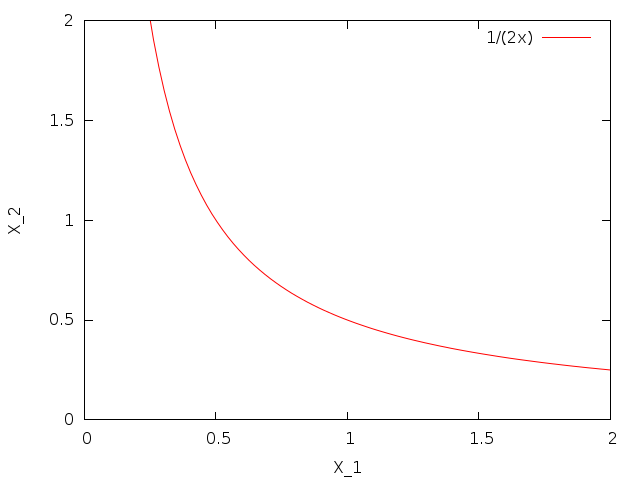
\includegraphics[scale=0.3]{graph.png}
\end{center}
\begin{align}
	B \cap M = \{(x_1, x_2) \in \mathbb{R}^2\ | (0 \leq x_1 \leq \frac{1}{4} \wedge 0 \leq x_2 \leq
	2) \vee (\frac{1}{4} \leq x_1 \leq 2 \wedge 0 \leq x_2 \leq \frac{1}{2x_1})\}\\
	\longrightarrow
	P(x_1x_2 \leq \frac{1}{2}) = \int^{\frac{1}{4}}_{0} \int^2_0 \frac{1}{4} dx_1dx_2
	+ \int^2_{\frac{1}{4}} \int^{\frac{1}{2x_1}}_0 \frac{1}{4} dx_2 dx_1
\end{align}
\subsection{Erwartungswert $\varepsilon$ diskreter Zufallsvariablen}
Falls der Erwartungswert einer diskreten Zufallsvariablen $X$ auf
einem diskreten Wahrscheinlichkeitsraum $(\Omega, \mathcal{A}, P)$ existiert,
ist
\begin{align}
	\varepsilon_P X = \sum_{\omega \in \Omega} X(\omega)P\{\omega\}
\end{align}

\section{Marginaldichte - Beispielrechnung}
\[	
	f(x_1,x_2)=
	\begin{cases}
		ce^{-(2x_1+3x_2)} & x_1  > 0 \: und \: 0 < x_2 <x_1 \\
		0 & sonst
	\end{cases}
\]
Marginaldichte:
\[
	\begin{split}
		f_1(x_1) 	& = \overbrace{\int_{0}^{x_1}}^{\text{Grenzen von }x_2} f(x_1,x_2) dx_2 \\
							  & = \int_{0}^{x_1} ce^{-2x_1}e^{-3x_2} \: dx_2 \\
						   & = \underbrace{c*e^{-2x_1}}_{\text{Konstante, da Integration nach} \: x_2}
		\overbrace{\int_{0}^{x_1} e^{-3x_2} \: dx_2}^{mit \: 0 \: und \: x_1 \: einsetzen \: integrieren} \\
		& = ce^{-2x_1}\, \frac{1}{3} (1-e^{-3x_2} )
	\end{split}
\]
Gegebenenfalls konnen wir das gleiche auch mit $dx_2$ tun wenn das einfach zur integrieren ist oder nach beiden Marginaldichten gefragt ist.
Damit $f(x_1,x_2)$ und $f_2(x_2)$ Dichten sind muss gelten:
\[
	\int f_2(x_2) dx_2 = 1
\]
bzw:
\[
	\int \int f(x_1,x_2) dx_1 dx_2 = 1
\]
\section{Transformation von Dichten}
\begin{center}
	\begin{tikzpicture}[
			bend angle=45,
			scale = 1.5,
			pre/.style={<-,shorten <=1pt,>=stealth',semithick},
			post/.style={->,shorten >=1pt,>=stealth',semithick},
			mid/.style={-,shorten >=1pt,>=stealth',semithick},
		place/.style={circle,draw=red!50,fill=red!20,thick}]

		\node[place]  (A) at ( 0,0)[label=above:Before] {$(\Omega, A, P) $};
		\node[place]  (B) at ( 2,0) {$(R^n, B_n, P^X)$}
		edge [pre] node [auto] {X} (A);
		\node[place, align=center]  (C) at ( 2,-3) {$(R^m, B_m, P^G$}
		edge [pre] node [auto] {$Y = G \circ X$} (A)
		edge [pre] node [auto] {$G$} (B);
	\end{tikzpicture}
\end{center}
\vspace*{7pt}
\textbf{Gegeben:} Man hat stochastisch unabhängige Zufallsvariablen $X_1, \ldots , X_n$ gegeben mit
Art der Verteilung.

\textbf{Gesucht:} Verteilung von Zufallsvariable $Y$, die sich aus $X_i$ berechnen lässt.

\textbf{Beispiel:}\\
Welche Verteilung besitzt
\begin{align}
	Y = \frac{X_1}{X_1 + X_2}
\end{align}
falls $X_1$ und $X_2$ exponentiell verteilt mit Paramter $\lambda$ und stochastisch
unabhängig sind.

\begin{enumerate}
	\item Wegen Unabhängigkeit der Variablen $X_1$ und $X_2$ besitzt $P^X$
		die Dichte $f(x_1,x_2) = f_1(x_1)f_2(x_2)$.
	\item $M = {(x_1, x_2); x_1 > 0 \text{ und } x_2 > 0}$\\
		$\longrightarrow$ Wertebereich von $x_n$ anhand von Verteilung ermitteln.
	\item Gleichungen  $G(x)$ definieren:
		\begin{align}
			y_1 &= \frac{x_1}{x_1 + x_2}\\
			y_2 &= x_2
		\end{align}
	\item Funktionaldeterminante ($J_{G}(x)$) der Abbildung $G$ berechnen
		\begin{align}
			J_{G}(x) =
			\text{det} \begin{pmatrix}
				\frac{\partial G_1}{\partial x_1} (x) & \cdots & \frac{\partial G_1}{\partial x_n} (x) \\
				\vdots  & \ddots & \vdots  \\
				\frac{\partial G_n}{\partial x_1} (x) & \cdots & \frac{\partial G_n}{\partial x_n} (x) \\
			\end{pmatrix}\\
			J_{G}(x_1,x_2) =
			\text{det} \begin{pmatrix}
				\frac{x_2}{(x_1 + x_2)^2} & * \\
				0 & 1 \\
			\end{pmatrix} = \frac{x_2}{(x_1 + x_2)^2}
		\end{align}
	\item Umkehrabbildung $G^*$ berechnen. Alle Zufallsvariablen werden
		werden mittels Funktionen verändert: z.B: $y_1 = x_1/x_2$.
		Jede i-te Funktion nach $x_i$ auflösen.
		\begin{align}
			x1 = \frac{y_1y_2}{1 - y_1}\\
			x_2 = y_2
		\end{align}
	\item Gesuchte Funktion: $g(y) = f(G^*(y))\frac{1}{|J_G(G^*(y))|}$\\
		$\longrightarrow$ Setze für alle $x_i$ dementsprechend $y_i$ ein und multipliziere
		mit Kehrwehrt von Funktionaldeterminante.
		\begin{align}
			g(y_1,y_2) = \lambda^2e^{-\frac{\lambda}{1 - y_1}}\frac{y_2}{(1-y_1)^2}
		\end{align}
	\item Mit Marginaldichte $g_1(y_1)$ berechnen:\\
		\begin{align}
			g_1(y_1) = \frac{\lambda}{1 - y_1} \int^\infty_0 y_2\frac{\lambda}{1 - y_1}
			e^{-\frac{\lambda}{1 - y_1}} dy_2\\
			= \frac{\lambda}{1 - y_1} m_1 (\varepsilon(\frac{\lambda}{1 - y_1}))\\
			= 1
		\end{align}
		$\longrightarrow$ Da Mittelwert der $\varepsilon$-Verteilung gerade Kehrwert des
		Paramters ist.
	\item Folgerung: Dichte $g_1$ ist also die der Uniform-Verteilung ($U(0,1)$).
\end{enumerate}

\end{document}
